% This is samplepaper.tex, a sample chapter demonstrating the
% LLNCS macro package for Springer Computer Science proceedings;
% Version 2.20 of 2017/10/04
%
\documentclass[runningheads]{llncs}
%
\usepackage{graphicx}
\usepackage{ctex}
\usepackage{xeCJK}
% Used for displaying a sample figure. If possible, figure files should
% be included in EPS format.
%
% If you use the hyperref package, please uncomment the following line
% to display URLs in blue roman font according to Springer's eBook style:
% \renewcommand\UrlFont{\color{blue}\rmfamily}

\begin{document}
%
\title{TEMCA:Temporal Element-wise Multiplication Cumsum Attention for 3d skeleton-based action recognition\thanks{Supported by organization x.}}
%
%\titlerunning{Abbreviated paper title}
% If the paper title is too long for the running head, you can set
% an abbreviated paper title here
%
\author{First Author\inst{1}\orcidID{0000-1111-2222-3333} \and
Second Author\inst{2,3}\orcidID{1111-2222-3333-4444} \and
Third Author\inst{3}\orcidID{2222--3333-4444-5555}}
%
\authorrunning{F. Author et al.}
% First names are abbreviated in the running head.
% If there are more than two authors, 'et al.' is used.
%
\institute{Princeton University, Princeton NJ 08544, USA \and
Springer Heidelberg, Tiergartenstr. 17, 69121 Heidelberg, Germany
\email{lncs@springer.com}\\
\url{http://www.springer.com/gp/computer-science/lncs} \and
ABC Institute, Rupert-Karls-University Heidelberg, Heidelberg, Germany\\
\email{\{abc,lncs\}@uni-heidelberg.de}}
%
\maketitle              % typeset the header of the contribution
%
\begin{abstract}
The abstract should briefly summarize the contents of the paper in
15--250 words.

\keywords{First keyword  \and Second keyword \and Another keyword.}
\end{abstract}
%
%
%
\section{Introduction}

Skeleton-based action recognition has emerged as a critical research 
direction in computer vision, driven by its applications in healthcare 
monitoring \cite{ntu}, human-computer interaction \cite{ntu120}, and surveillance systems \cite{ref3}.



The advent of Graph Convolutional Networks (GCNs) \cite{ref8} revolutionized the field by 
explicitly modeling skeletal topology through adjacency matrices. Pioneering 
work like ST-GCN \cite{ref7} introduced spatial-temporal convolutions to jointly 
capture joint correlations across frames. Subsequent innovations proposed 
learnable adjacency matrices \cite{ref9,ref10} and multi-scale aggregation 
strategies \cite{multiscale} to enhance flexibility.Despite these advancements, 
two critical limitations persist: (1) While existing works predominantly focus on spatial topology modeling,
the temporal feature extraction relies on multi-scale convolutions 
that inadequately capture contextual dependencies across time. (2) Fixed prior topology inputs
enforce a static inductive bias that restricts the network's ability to discover latent action-specific correlations.


Therefore, this paper proposes a novel architecture that advances skeleton-based action recognition through three pivotal innovations:


First, we introduce a Temporal Element-wise Multiplication Cumsum 
Attention (TEMCA) mechanism to address temporal contextualization. 
While temporal modeling remains pivotal for skeleton-based action 
recognition, existing approaches predominantly rely on multi-scale temporal convolution modules \cite{ref9,ref10,ref11,ref12} that lack specialized architectural design for capturing complex temporal dependencies. To address this, we draw inspiration from the Token Statistic Transformer \cite{tost} to devise a multi-scale linear attention mechanism. Our TEMCA employs dilated context windows to 
establish hierarchical receptive fields, explicitly capturing both 
local motion nuances and global phase transitions. 
%这一段看字数不够加上去
%This contrasts 
%with conventional temporal convolutions in GCNs, whose rigid filter 
%designs and linear aggregation strategies struggle to model 
%non-sequential temporal relationships across action stages.

%这个部分我不知道详细的实现,需要手动改一下
Second, inspired by the activation-free method \cite{rewrite_stars}, we fundamentally redesign self-attention computation through activation-free element-wise multiplication, resolving the efficiency bottleneck of temporal modeling. 
While preserving attention's dynamic weighting capability, TEMCA 
accelerates training convergence compared to standard 
ToST variants, yet maintains state-of-the-art accuracy. 

%这一段话不够再加
%This innovation proves particularly critical for skeleton sequences, 
%where temporal relationships require lightweight yet expressive 
%operators.

Third, we propose a multi-modal skeleton representation through latent 
topology discovery via line-graph augmentation. While multi-modal 
learning, such as joint-bone ensembles \cite{ref9,ref10,ref11,ref13} has proven 
effective in mitigating rigid structural priors, existing methods rely 
on simplistic feature engineering, training separate models on linearly 
transformed joint coordinates for late fusion. 
Building on this paradigm, we introduce line-graph augmentation, a 
novel skeletal modality that explicitly encodes angular kinematics 
between adjacent bones. The ensemble of line-graph has been demonstrated 
to capture richer semantic information, effectively boosting prediction 
accuracy.




\subsubsection{Sample Heading (Third Level)} Only two levels of
headings should be numbered. Lower level headings remain unnumbered;
they are formatted as run-in headings.

\paragraph{Sample Heading (Fourth Level)}
The contribution should contain no more than four levels of
headings. Table~\ref{tab1} gives a summary of all heading levels.

\begin{table}
\caption{Table captions should be placed above the
tables.}\label{tab1}
\begin{tabular}{|l|l|l|}
\hline
Heading level &  Example & Font size and style\\
\hline
Title (centered) &  {\Large\bfseries Lecture Notes} & 14 point, bold\\
1st-level heading &  {\large\bfseries 1 Introduction} & 12 point, bold\\
2nd-level heading & {\bfseries 2.1 Printing Area} & 10 point, bold\\
3rd-level heading & {\bfseries Run-in Heading in Bold.} Text follows & 10 point, bold\\
4th-level heading & {\itshape Lowest Level Heading.} Text follows & 10 point, italic\\
\hline
\end{tabular}
\end{table}


\noindent Displayed equations are centered and set on a separate
line.
\begin{equation}
x + y = z
\end{equation}
Please try to avoid rasterized images for line-art diagrams and
schemas. Whenever possible, use vector graphics instead (see
Fig.~\ref{fig1}).

\begin{figure}
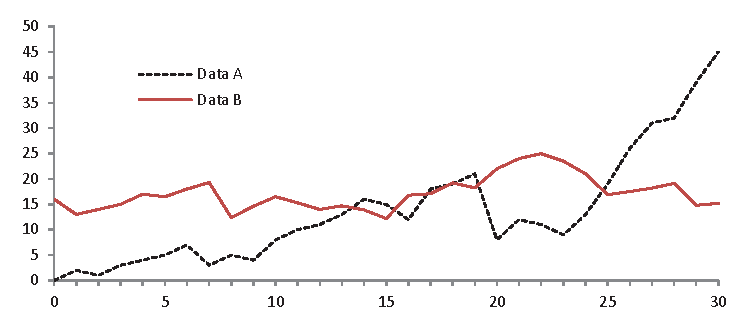
\includegraphics[width=\textwidth]{fig1.eps}
\caption{A figure caption is always placed below the illustration.
Please note that short captions are centered, while long ones are
justified by the macro package automatically.} \label{fig1}
\end{figure}

\begin{theorem}
This is a sample theorem. The run-in heading is set in bold, while
the following text appears in italics. Definitions, lemmas,
propositions, and corollaries are styled the same way.
\end{theorem}
%
% the environments 'definition', 'lemma', 'proposition', 'corollary',
% 'remark', and 'example' are defined in the LLNCS documentclass as well.
%
\begin{proof}
Proofs, examples, and remarks have the initial word in italics,
while the following text appears in normal font.
\end{proof}
For citations of references, we prefer the use of square brackets
and consecutive numbers. Citations using labels or the author/year
convention are also acceptable. The following bibliography provides
a sample reference list with entries for journal
articles~\cite{ref_article1}, an LNCS chapter~\cite{ref_lncs1}, a
book~\cite{ref_book1}, proceedings without editors~\cite{ref_proc1},
and a homepage~\cite{ref_url1}. Multiple citations are grouped
\cite{ref_article1,ref_lncs1,ref_book1},
\cite{ref_article1,ref_book1,ref_proc1,ref_url1}.
%

% 添加 BibTeX 引用指令
\bibliographystyle{splncs04}
\bibliography{references}

\end{document}
